\chapter{Examples}
\label{cha:examples}

\section{Solving nonlinear equations}
\label{sec:nonlinear-equations}

\feel allows to solve nonlinear equations thanks to its interface to
the interface to the PETSc nonlinear solver library. It requires the
implementation of two extra functions in your application that will
update the jacobian matrix associated to the tangent problem and the
residual.

Consider that you have an application class \lstinline!MyApp! with a
backend as data member
\begin{lstlisting}{gobble=2}
#include <feel/feelcore/feel.hpp>
#include <feel/feelcore/application.hpp>
#include <feel/feelalg/backend.hpp>
namespace Feel {

class MyApp : public Application
{
  public:

  typedef Backend<double> backend_type;
  typedef boost::shared_ptr<backend_type> backend_ptrtype;

  MyApp( int argc, char** argv,
  AboutData const& ad, po::options_description const& od )
  :
  // init the parent class
  Application( argc, argv, ad, od ),
  // init the backend
  M_backend( backend_type::build( this->vm() ) ),
  {
    // define the callback functions (works only for the PETSc backend)
    M_backend->nlSolver()->residual =
      boost::bind( &self_type::updateResidual, boost::ref( *this ), _1, _2 );
    M_backend->nlSolver()->jacobian =
      boost::bind( &self_type::updateJacobian, boost::ref( *this ), _1, _2 );

  }
  void updateResidual( const vector_ptrtype& X, vector_ptrtype& R )
  {
    // update the matrix J (Jacobian matrix) associated
    // with the tangent problem
  }
  void updateJacobian( const vector_ptrtype& X, sparse_matrix_ptrtype& J)
  {
    // update the vector R associated with the residual
  }
  void run()
  {

    //define space
    Xh...
    element_type u(Xh);
    // initial guess is 0
    u = project( M_Xh, elements(mesh), constant(0.) );
    vector_ptrtype U( M_backend->newVector( u.functionSpace() ) );
    *U = u;

    // define R and J
    vector_ptrtype R( M_backend->newVector( u.functionSpace() ) );
    sparse_matrix_ptrtype J;

    // update R
    updateJacobian( U, R );
    // update J
    updateResidual( U, J );

    // solve using non linear methods (newton)
    // tolerance : 1e-10
    // max number of iterations : 10
    M_backend->nlSolve( J, U, R, 1e-10, 10 );

    // the soluution was stored in U
    u = *U;
  }
  private:

  backend_ptrtype M_backend;
};
} // namespace Feel
\end{lstlisting}

The function \lstinline!updateJacobian! and \lstinline!updateResidual!
implement the assmebly of the matrix $J$ (jacobian matrix) and the
vector $R$ (residual vector) respectively.

\subsection{A first nonlinear problem}
\label{sec:bratu}

As a simple example, let $\Omega$ be a subset of $\mathbb{R}^d, d=1,2,3$,
(\emph{i.e.} $\Omega=[-1,1]^d$) with boundary $\partial
\Omega$. Consider now the following equation and boundary condition
\begin{equation}
  \label{eq:29}
  -\Delta u + u^\lambda = f,\quad u = 0 \text{ on } \partial \Omega.
\end{equation}
where $\lambda \in \mathbb{R_+}$ is a given parameter and $f=1$.


\begin{nota}
  To be described in this section. For now see
  \texttt{doc/tutorial/nonlinearpow.cpp} for an implementation of this
  problem.
\end{nota}

\subsection{Simplified combustion problem: Bratu}
\label{sec:bratu}

As a simple example, let $\Omega$ be a subset of $\mathbb{R}^d, d=1,2,3$,
(\emph{i.e.} $\Omega=[-1,1]^d$) with boundary $\partial
\Omega$. Consider now the following equation and boundary condition
\begin{equation}
  \label{eq:29}
  -\Delta u + \lambda e^u = f,\quad u = 0 \text{ on } \partial \Omega
\end{equation}
where $\lambda$ is a given parameter. Ceci est généralement appellé le
problème de Bratu et apparaît lors de la simplification de modèles de
processus de diffusion non-linéaires par exemple dans le domaine de la
combustion.

\begin{nota}
  To be described in this section. For now see
  \texttt{doc/tutorial/bratu.cpp} for an implementation of this
  problem.
\end{nota}

\newcommand{\Gr}{\ensuremath{\mathrm{Gr}\xspace}}
\renewcommand{\Pr}{\ensuremath{\mathrm{Pr}\xspace}}

\section{Natural convection in a heated tank}


\subsection{Description}
\label{sec:description}

The goal of this project is to simulate the fluid flow under natural
convection: the heated fluid circulates towards the low temperature
under the action of density and gravity differences. Thie phenomenon
is important in the sense it models evacuation of heat, generated by
friction forces for example, with  a cooling fluid.

We shall put in place a simple convection problem in order to study
the phenomenon without having to handle the difficulties of more
complex domaines. We describe then some necessary transformations to
the equations, then we define quantities of interest to be able to
compare the simulations with different parameter values.


\newcommand{\Water}{\text{\textsc{Water}}\xspace}
\newcommand{\Fluid}{\text{\textsc{Fluid}}\xspace}
\tikzstyle{snakearrow} = [decoration={snake,aspect=0.2,segment length=1cm,amplitude=1mm},decorate]

\begin{figure}[htbp]
  \centering
  \begin{tikzpicture}[thick,scale=5]

    %% draw axis
    \draw[->] (-0.6,-0.4) -- (1.1,-0.4) node[right] {$x$} coordinate (x axis);
    \draw[-] (-0.,-0.39) -- (0,-0.41) node[below] {$0$};
    \draw[-] (1.,-0.39) -- (1,-0.41) node[below] {$W$};
    \draw[->] (-0.4,-0.6) -- (-0.4,1.1) node[above] {$y$} coordinate (y axis);
    \draw[-] (-0.39,-0.) -- (-0.41,-0.) node[left] {$0$};
    \draw[-] (-0.39,1.) -- (-0.41,1) node[left] {$1$};

    %% draw top and down walls
    \fill[pattern={north east lines},pattern color=blue] (0,1) rectangle  (1,1.02) ;
    \fill[pattern={north west lines},pattern color=blue] (0,0) rectangle  (1,-0.02) ;

    %% Draw the domain
    \draw[very thick,fill=blue!10!white,draw=blue!50] (0,0) rectangle  (1,1) ;
    \node at (0.1,0.5) {$\Gamma_1$};
    \node at (0.5,0.1) {$\Gamma_2$};
    \node at (0.9,0.5)  {$\Gamma_3$};
    \node at (0.8,0.9)  {$\Gamma_4$};
    \node (omega) at (0.5,0.3)  {$\Omega (\Fluid)$};
    % \draw[->,snakearrow] (omega) -- (0.5,0.5);
    \draw[<->] (0,-0.1) -- (1,-0.1) node [below,midway] {$W$};
    \draw[-] (0.5,1.) -- (0.5,0.5) node[left,midway] {$\Gamma_f$};
    \draw[-,ultra thick,color=blue] (0,0) -- (0,1) node [left,midway] {$T_0$};
    \draw[-,ultra thick,color=red] (1,0) -- (1,1)  {};


    \foreach \y in {0.1,0.3,0.5,0.7,0.9} {
      %%\draw[->] (\x, -1.5) -- (\x,\pgfmathqparse{-0.7*\x*\x+0.7*8*\x-12} \pgfmathresult);
      %%\pgfmathsetmacro{\pgf@x}{\x}
      %%\pgfmathparse{-0.7*\pgf@x*\pgf@x+0.7*8*\pgf@x-0.7*12}
      %%\def\y{\pgfmathresult}
      \def\x{1.3}
      \draw[->] (1.3, \y) -- (1.1,\y);
    }
    \node at (1.6,0.5) {Heat flux};

  \end{tikzpicture}
  \caption{Geometry of the model}
  \label{fig:heatns:1}
\end{figure}

To study the convection, we use a model problem: it consists in a
rectangular tank of height $1$ and width $W$, in which the fluid is
enclosed, see figure~\ref{fig:heatns:1}. We wish to know the fluid velocity
$\mathbf{u}$, the fluid pressure $p$ and fluid temperature $\theta$.

We introduce the adimensionalized Navier-Stokes and heat equations
parametrized by the Grashof and Prandtl numbers. These parameters
allow to describe the various regimes of the fluid flow and heat
transfer in the tank when varying them.

The adimensionalized steady incompressible Navier-Stokes equations reads:
\begin{equation}
  \label{eq:38}
  \begin{split}
    \mathbf{u}\cdot\nabla \mathbf{u} +\nabla p -\frac{1}{\sqrt{\Gr}} \Delta \mathbf{u} &= \theta \mathbf{e}_2\\
    \nabla \cdot \mathbf{u} & = 0\ \text{sur}\ \Omega\\
    \mathbf{u} & = \mathbf{0}\ \text{sur}\ \partial \Omega
  \end{split}
\end{equation}
where $\Gr$ is the Grashof number, $\mathbf{u}$ the adimensionalized
velocity and $p$ adimensionalized pressure and $\theta$ the
adimensionalized temperature. The temperature is in fact the
difference between the temperature in the tank and the temperature
$T_0$ on boundary $\Gamma_1$.

The heat equation reads:
\begin{equation}
  \label{eq:37}
  \begin{split}
    \mathbf{u} \cdot \nabla \theta -\frac{1}{\sqrt{\Gr}\Pr} \Delta \theta &= 0\\
    \theta &= 0\ \text{sur}\ \Gamma_1\\
    \frac{\partial \theta}{\partial n} &= 0\ \text{sur}\ \Gamma_{2,4}\\
    \frac{\partial \theta}{\partial n} &= 1\ \text{sur}\ \Gamma_3
  \end{split}
\end{equation}
where $\Pr$ is the Prandtl number.

% \subsection{Nombre de Grashof}
% \label{sec:nombre-de-grashof}
% Le nombre de Grashof (\Gr) est un nombre sans dimension utilisé en
% mécanique des fluides pour caractériser la convection libre dans un
% fluide. Il correspond au rapport des forces de gravité sur les forces
% visqueuses.

% On le définit de la manière suivante
% \begin{equation}
%   \label{eq:18}
%   \Gr = \frac{g\  \beta\  (T-T_\infty)\  {L_c}^3}{\nu^2}
% \end{equation}
% avec:
% \begin{itemize}
% \item $g$ - constante gravitationnelle
% \item $\beta$ - coefficient de dilatation
% \item $T-T_\infty$ - différence de température
% \item $L_c$ - longueur caractéristique
% \item $\nu$ - viscosité cinématique
% \end{itemize}

% \subsection{Nombre de Prandtl}
% \label{sec:nombre-de-prandtl}

% Le nombre de Prandtl (\Pr) est un nombre sans dimension. Il représente
% le rapport entre la diffusivité de quantité de mouvement $\nu$ (ou
% viscosité cinématique) et la diffusivité thermique.

% On le définit de la manière suivante
% \begin{equation}
%   \label{eq:19}
%   \Pr=\frac {\mu C_p }{\lambda}=\frac {\mu}{\frac {k}{C_p}}=\frac {\frac {\mu}{\rho}}{\frac {k}{\rho C_p}}=\frac {\nu}{\alpha}
% \end{equation}
% avec
% \begin{itemize}
% \item $\nu$ la viscosité cinématique en $m^2\cdot s^{-1}$
% \item $\rho$ la masse volumique en $kg\cdot m^{-3}$
% \item $\alpha$ la diffusivité thermique en $m^2\cdot s^{-1}$
% \item $\mu$ la viscosité dynamique en $N\cdot s\cdot m^{-2}$
% \item $C_p$ la chaleur massique en $J\cdot kg^{-1}\cdot K^{-1}$
% \item $k$ la conductivité thermique $W \cdot m^{-1}\cdot K^{-1}$
% \end{itemize}



\subsection{Influence of parameters}
\label{sec:infl-des-param}


what are the effects of the Grashof and Prandtl numbers ? We remark
that both terms with these parameters appear in front of the $\Delta$
parameter, they thus act on the diffusive terms. If we increase the
Grashof number or the Prandtl number the coefficients multiplying the
diffusive terms decrease, and this the convection, that is to say the
transport of the heat via the fluid, becomes dominant. This leads also
to a more difficult and complex flows to simulate, see
figure~\ref{fig:heatns:2}. The influence of the Grashof and Prandtl
numbers are different but they generate similar difficulties and flow
configurations. Thus we look only here at the influence of the Grashof
number which shall vary in $[1, 1e7]$.

\begin{figure}[htbp]
  \centering
  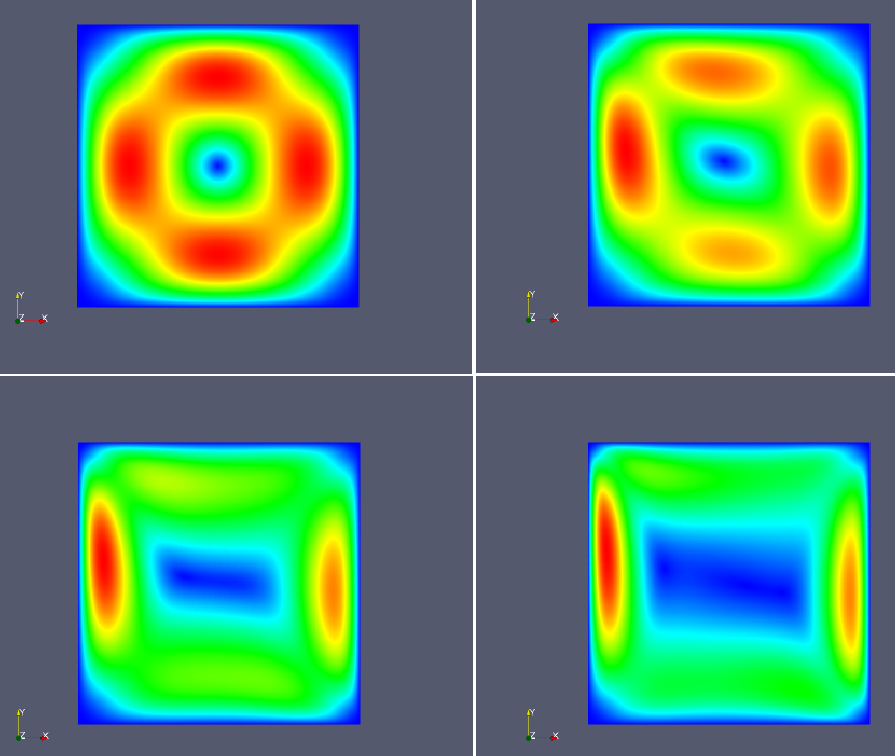
\includegraphics[width=.8\linewidth]{pngs/flow_grashof}
  \caption{Velocity norm with respect to  Grashof, $\Gr=100, 10000,
    100000, 500000$. $h=0.01$ and $\Pr=1$.}
  \label{fig:heatns:2}
\end{figure}

\subsection{Quantities of interest}
\label{sec:quant-du-benchm}

We would like to compare the results of many simulations with respect
to the Grashof defined in the previous section. We introduce two
quantities which will allow us to observe the behavior of the flow and
heat transfer.


\subsubsection{Mean temperature}
\label{sec:mean-temperature}

We consider first the mean temperature on boundary $\Gamma_3$
\begin{equation}
  \label{eq:16}
  T_3 = \int_{\Gamma_3} \theta
\end{equation}

This quantity should decrease with increasing Grashof because the
fluid flows faster and will transport more heat which will cool down
the heated boundary $\Gamma_3$. We observe this behavior on the
figure~\ref{fig:heatns:3}.

\begin{figure}[htbp]
  \centering
  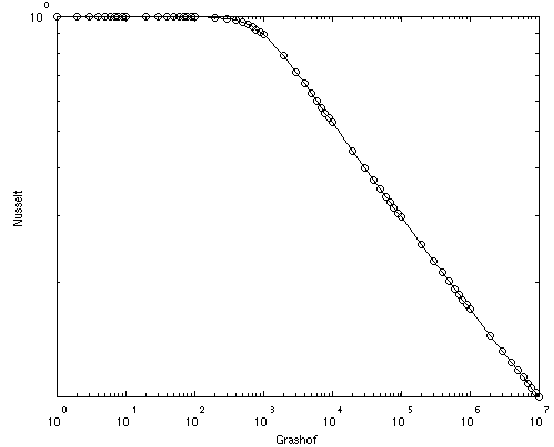
\includegraphics[width=.8\linewidth]{pngs/temp_grashof}
  \caption{Mean temperature with respect to the Grashof number;
    $h=0.02$ with $\mathbb{P}_3$ Lagrange element for the velocity,
    $\mathbb{P}_2$ Lagrange for the pressure and $\mathbb{P}_1$
    Lagrange for the temperature.}
  \label{fig:heatns:3}
\end{figure}

\subsubsection{Flow rate}
\label{sec:flow-rate}

Another quantity of interest is the flow rate through the middle of the
tank. We define a segment $\Gamma_f$ as being the vertical top
semi-segment located at $W/2$ with height $1/2$, see
figure~\ref{fig:heatns:1}. The flow rate, denoted $\mathrm{D}_f$, reads
\begin{equation}
  \label{eq:17}
  \mathrm{D}_f =  \int_{\Gamma_f} \mathbf{u} \cdot \mathbf{e}_1
\end{equation}
where $\mathbf{e}_1=(1,0)$. Note that the flow rate can be negative or
positive depending on the direction in which the fluid flows.

As a function of the Grashof, we shall see a increase in the flow
rate. This is true for small Grashof, but starting at $1e3$ the flow
rate decreases. The fluid is contained in a boundary layer which is
becoming smaller as the Grashof increases.

\begin{figure}[htbp]
  \centering
  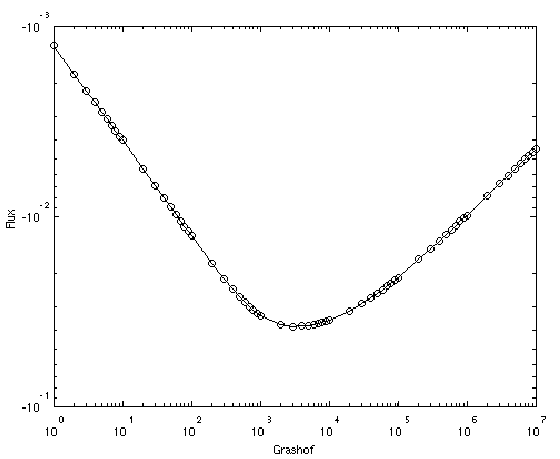
\includegraphics[width=.8\linewidth]{pngs/debit_grashof}
  \caption{Behavior of the flow rate with respect to the Grashof number; $h = 0.02$,
    $\mathbb{P}_3$ for the velocity, $\mathbb{P}_2$ for the pressure and
    $\mathbb{P}_1$ for the temperature.}
  \label{fig:4}
\end{figure}

\subsection{Implementation}
\label{sec:implementation}

This application in implemented in
\texttt{life/doc/tutorial/convection*.cpp}. The implementation solve
the full nonlinear problem using the nonlinear solver framework.

